% Created by tikzDevice version 0.10.1 on 2016-06-30 12:15:51
% !TEX encoding = UTF-8 Unicode
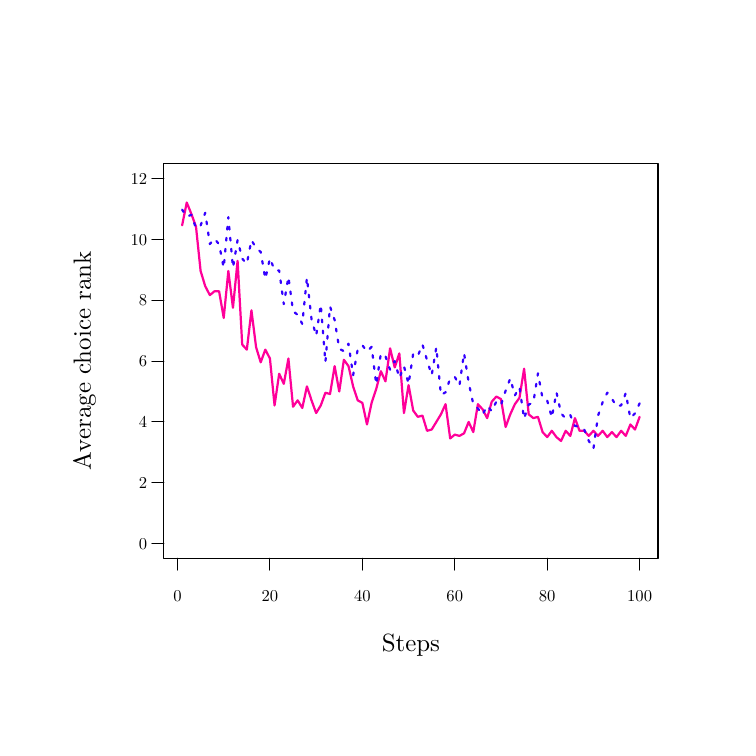
\begin{tikzpicture}[x=1pt,y=1pt]
\definecolor{fillColor}{RGB}{255,255,255}
\path[use as bounding box,fill=fillColor,fill opacity=0.00] (0,0) rectangle (252.94,252.94);
\begin{scope}
\path[clip] ( 49.20, 61.20) rectangle (227.75,203.75);
\definecolor{drawColor}{RGB}{255,0,153}

\path[draw=drawColor,line width= 0.8pt,line join=round,line cap=round] ( 55.81,181.51) --
	( 57.48,189.76) --
	( 59.15,185.63) --
	( 60.82,181.05) --
	( 62.49,165.01) --
	( 64.16,159.51) --
	( 65.83,156.30) --
	( 67.50,157.68) --
	( 69.17,157.68) --
	( 70.84,148.05) --
	( 72.51,165.01) --
	( 74.18,151.72) --
	( 75.85,168.68) --
	( 77.52,138.43) --
	( 79.19,136.60) --
	( 80.86,150.80) --
	( 82.53,137.51) --
	( 84.20,132.01) --
	( 85.87,136.60) --
	( 87.54,133.39) --
	( 89.21,116.43) --
	( 90.88,127.89) --
	( 92.55,124.22) --
	( 94.22,133.39) --
	( 95.89,115.97) --
	( 97.56,118.27) --
	( 99.23,115.52) --
	(100.90,123.31) --
	(102.57,118.27) --
	(104.24,113.68) --
	(105.91,116.43) --
	(107.58,121.02) --
	(109.25,120.56) --
	(110.92,130.64) --
	(112.59,121.47) --
	(114.26,132.93) --
	(115.93,130.64) --
	(117.60,123.31) --
	(119.27,118.27) --
	(120.94,117.35) --
	(122.61,109.56) --
	(124.28,117.35) --
	(125.95,122.39) --
	(127.62,128.81) --
	(129.29,125.14) --
	(130.96,137.06) --
	(132.63,130.18) --
	(134.30,135.22) --
	(135.97,113.68) --
	(137.64,123.77) --
	(139.31,114.60) --
	(140.98,112.31) --
	(142.65,112.77) --
	(144.32,107.27) --
	(145.99,107.73) --
	(147.66,110.47) --
	(149.33,113.22) --
	(151.00,116.89) --
	(152.67,104.52) --
	(154.34,105.89) --
	(156.01,105.43) --
	(157.68,106.35) --
	(159.35,110.47) --
	(161.02,106.81) --
	(162.69,116.89) --
	(164.36,115.06) --
	(166.03,111.85) --
	(167.70,117.81) --
	(169.37,119.64) --
	(171.04,118.72) --
	(172.71,108.64) --
	(174.38,113.22) --
	(176.05,116.89) --
	(177.71,119.18) --
	(179.38,129.72) --
	(181.05,113.22) --
	(182.72,111.85) --
	(184.39,112.31) --
	(186.06,106.81) --
	(187.73,104.98) --
	(189.40,107.27) --
	(191.07,104.98) --
	(192.74,103.60) --
	(194.41,107.27) --
	(196.08,105.43) --
	(197.75,111.85) --
	(199.42,107.27) --
	(201.09,107.27) --
	(202.76,105.43) --
	(204.43,107.27) --
	(206.10,105.43) --
	(207.77,107.27) --
	(209.44,104.98) --
	(211.11,106.81) --
	(212.78,104.98) --
	(214.45,107.27) --
	(216.12,105.43) --
	(217.79,109.56) --
	(219.46,107.73) --
	(221.13,112.31);
\end{scope}
\begin{scope}
\path[clip] (  0.00,  0.00) rectangle (252.94,252.94);
\definecolor{drawColor}{RGB}{0,0,0}

\path[draw=drawColor,line width= 0.4pt,line join=round,line cap=round] ( 54.14, 61.20) -- (221.13, 61.20);

\path[draw=drawColor,line width= 0.4pt,line join=round,line cap=round] ( 54.14, 61.20) -- ( 54.14, 56.92);

\path[draw=drawColor,line width= 0.4pt,line join=round,line cap=round] ( 87.54, 61.20) -- ( 87.54, 56.92);

\path[draw=drawColor,line width= 0.4pt,line join=round,line cap=round] (120.94, 61.20) -- (120.94, 56.92);

\path[draw=drawColor,line width= 0.4pt,line join=round,line cap=round] (154.34, 61.20) -- (154.34, 56.92);

\path[draw=drawColor,line width= 0.4pt,line join=round,line cap=round] (187.73, 61.20) -- (187.73, 56.92);

\path[draw=drawColor,line width= 0.4pt,line join=round,line cap=round] (221.13, 61.20) -- (221.13, 56.92);

\node[text=drawColor,anchor=base,inner sep=0pt, outer sep=0pt, scale=  0.60] at ( 54.14, 45.60) {0};

\node[text=drawColor,anchor=base,inner sep=0pt, outer sep=0pt, scale=  0.60] at ( 87.54, 45.60) {20};

\node[text=drawColor,anchor=base,inner sep=0pt, outer sep=0pt, scale=  0.60] at (120.94, 45.60) {40};

\node[text=drawColor,anchor=base,inner sep=0pt, outer sep=0pt, scale=  0.60] at (154.34, 45.60) {60};

\node[text=drawColor,anchor=base,inner sep=0pt, outer sep=0pt, scale=  0.60] at (187.73, 45.60) {80};

\node[text=drawColor,anchor=base,inner sep=0pt, outer sep=0pt, scale=  0.60] at (221.13, 45.60) {100};

\path[draw=drawColor,line width= 0.4pt,line join=round,line cap=round] ( 49.20, 66.48) -- ( 49.20,198.47);

\path[draw=drawColor,line width= 0.4pt,line join=round,line cap=round] ( 49.20, 66.48) -- ( 44.92, 66.48);

\path[draw=drawColor,line width= 0.4pt,line join=round,line cap=round] ( 49.20, 88.48) -- ( 44.92, 88.48);

\path[draw=drawColor,line width= 0.4pt,line join=round,line cap=round] ( 49.20,110.47) -- ( 44.92,110.47);

\path[draw=drawColor,line width= 0.4pt,line join=round,line cap=round] ( 49.20,132.47) -- ( 44.92,132.47);

\path[draw=drawColor,line width= 0.4pt,line join=round,line cap=round] ( 49.20,154.47) -- ( 44.92,154.47);

\path[draw=drawColor,line width= 0.4pt,line join=round,line cap=round] ( 49.20,176.47) -- ( 44.92,176.47);

\path[draw=drawColor,line width= 0.4pt,line join=round,line cap=round] ( 49.20,198.47) -- ( 44.92,198.47);

\node[text=drawColor,anchor=base east,inner sep=0pt, outer sep=0pt, scale=  0.60] at ( 43.20, 64.41) {0};

\node[text=drawColor,anchor=base east,inner sep=0pt, outer sep=0pt, scale=  0.60] at ( 43.20, 86.41) {2};

\node[text=drawColor,anchor=base east,inner sep=0pt, outer sep=0pt, scale=  0.60] at ( 43.20,108.41) {4};

\node[text=drawColor,anchor=base east,inner sep=0pt, outer sep=0pt, scale=  0.60] at ( 43.20,130.41) {6};

\node[text=drawColor,anchor=base east,inner sep=0pt, outer sep=0pt, scale=  0.60] at ( 43.20,152.40) {8};

\node[text=drawColor,anchor=base east,inner sep=0pt, outer sep=0pt, scale=  0.60] at ( 43.20,174.40) {10};

\node[text=drawColor,anchor=base east,inner sep=0pt, outer sep=0pt, scale=  0.60] at ( 43.20,196.40) {12};

\path[draw=drawColor,line width= 0.4pt,line join=round,line cap=round] ( 49.20, 61.20) --
	(227.75, 61.20) --
	(227.75,203.75) --
	( 49.20,203.75) --
	( 49.20, 61.20);
\end{scope}
\begin{scope}
\path[clip] (  0.00,  0.00) rectangle (252.94,252.94);
\definecolor{drawColor}{RGB}{0,0,0}

\node[text=drawColor,anchor=base,inner sep=0pt, outer sep=0pt, scale=  0.90] at (138.47, 27.60) {Steps};

\node[text=drawColor,rotate= 90.00,anchor=base,inner sep=0pt, outer sep=0pt, scale=  0.90] at ( 22.80,132.47) {Average choice rank};
\end{scope}
\begin{scope}
\path[clip] ( 49.20, 61.20) rectangle (227.75,203.75);
\definecolor{drawColor}{RGB}{51,0,255}

\path[draw=drawColor,line width= 0.8pt,dash pattern=on 1pt off 3pt ,line join=round,line cap=round] ( 55.81,187.18) --
	( 57.48,184.61) --
	( 59.15,185.32) --
	( 60.82,180.47) --
	( 62.49,181.47) --
	( 64.16,186.04) --
	( 65.83,174.75) --
	( 67.50,176.75) --
	( 69.17,174.61) --
	( 70.84,166.18) --
	( 72.51,184.47) --
	( 74.18,166.18) --
	( 75.85,176.18) --
	( 77.52,169.47) --
	( 79.19,167.61) --
	( 80.86,176.18) --
	( 82.53,173.33) --
	( 84.20,171.90) --
	( 85.87,162.18) --
	( 87.54,169.61) --
	( 89.21,165.33) --
	( 90.88,165.18) --
	( 92.55,153.04) --
	( 94.22,162.90) --
	( 95.89,150.47) --
	( 97.56,149.19) --
	( 99.23,145.90) --
	(100.90,162.61) --
	(102.57,147.61) --
	(104.24,141.61) --
	(105.91,152.90) --
	(107.58,132.04) --
	(109.25,152.18) --
	(110.92,147.33) --
	(112.59,136.90) --
	(114.26,136.04) --
	(115.93,138.76) --
	(117.60,127.33) --
	(119.27,136.76) --
	(120.94,138.19) --
	(122.61,135.90) --
	(124.28,137.61) --
	(125.95,124.04) --
	(127.62,135.19) --
	(129.29,134.19) --
	(130.96,129.33) --
	(132.63,132.47) --
	(134.30,126.33) --
	(135.97,130.62) --
	(137.64,124.19) --
	(139.31,135.19) --
	(140.98,134.33) --
	(142.65,138.47) --
	(144.32,132.76) --
	(145.99,127.33) --
	(147.66,137.47) --
	(149.33,120.19) --
	(151.00,121.19) --
	(152.67,126.19) --
	(154.34,126.76) --
	(156.01,123.62) --
	(157.68,135.33) --
	(159.35,124.76) --
	(161.02,116.90) --
	(162.69,115.33) --
	(164.36,113.05) --
	(166.03,116.33) --
	(167.70,114.33) --
	(169.37,117.90) --
	(171.04,116.62) --
	(172.71,121.76) --
	(174.38,126.19) --
	(176.05,120.05) --
	(177.71,123.04) --
	(179.38,111.62) --
	(181.05,116.76) --
	(182.72,117.47) --
	(184.39,128.04) --
	(186.06,118.90) --
	(187.73,118.19) --
	(189.40,112.05) --
	(191.07,121.19) --
	(192.74,113.62) --
	(194.41,111.62) --
	(196.08,112.90) --
	(197.75,109.05) --
	(199.42,108.76) --
	(201.09,107.76) --
	(202.76,103.62) --
	(204.43,100.76) --
	(206.10,112.76) --
	(207.77,117.62) --
	(209.44,121.05) --
	(211.11,118.90) --
	(212.78,116.05) --
	(214.45,116.47) --
	(216.12,120.90) --
	(217.79,111.76) --
	(219.46,113.62) --
	(221.13,117.19);
\end{scope}
\end{tikzpicture}
